\section{Triviality of Snarks}\label{sec:snarks-triviality}

As mentioned earlier, some authors use the term \quotes{nontrivial} when defining snarks. One of the attributes linked to the triviality of snarks is the containment of a digon, a graph with two vertices connected by two edges. Consider a graph $G$ with a digon. Let $G'$~be a~graph obtained by removing the digon, as shown in \cref{fig:trivial-digon}. The graph $G$ is colourable if and only if $G'$ is colourable.

\begin{figure}
	\centering
	\begin{tikzpicture}[every node/.style={draw,circle,very thick, fill=black}]
	
	\node[draw=none, fill=none] (1) at (0,0) {};
	\node (2) at (1,0) {};
	\node (3) at (4,0) {};
	\node[draw=none, fill=none] (4) at (5,0) {};
	
	\path (1) edge (2);
	\path (2) edge[bend left] (3);
	\path (2) edge[bend right] (3);
	\path (3) edge (4);
	
	\node[draw=none, fill=none] (arrow) at (7, 0) {$\rightarrow$};
	
	\node[draw=none, fill=none] (5) at (9,0) {};
	\node[draw=none, fill=none] (6) at (14,0) {};
	
	\path (5) edge (6);
	
	
	
\end{tikzpicture}
	\caption{Replacement of a digon in a snark}
	\label{fig:trivial-digon}
\end{figure}

 If a cubic graph $G$ contains a triangle, it can be replaced with a single vertex resulting in a smaller graph $G'$ as visualised in \cref{fig:trivial-triangle}. As with digons, $G$ is colourable if and only if $G'$ is colourable.
 
 \begin{figure}
 	\centering
 	\begin{subfigure}{0.4\textwidth}
 		\raggedleft
 		\begin{tikzpicture}[every node/.style={draw,circle,very thick, fill=black}]
	
	\graph[clockwise, radius=2cm, nodes={draw=none, fill=none}, edges={draw=none}, empty nodes] {subgraph C_n [n=3,name=B] };
	
	\graph[clockwise, radius=1cm, empty nodes] {subgraph C_n [n=3,name=A] };
	
	\foreach \i in {1,2,3}{
		\draw (A \i) -- (B \i);
	}

	
	
\end{tikzpicture}
 	\end{subfigure}
 	\hfill
 	\begin{subfigure}{0.1\textwidth}
 		\centering
 		$\rightarrow$
 		\newline\newline
 	\end{subfigure}
 	\hfill
 	\begin{subfigure}{0.4\textwidth}
 		\raggedright
 		\begin{tikzpicture}[every node/.style={draw,circle,very thick, fill=black}]
	
	\graph[clockwise, radius=2cm, nodes={draw=none, fill=none}, edges={draw=none}, empty nodes] {subgraph C_n [n=3,name=B] };
	
	\graph[clockwise, radius=0cm, empty nodes] {subgraph C_n [n=3,name=A] };
	
	\foreach \i in {1,2,3}{
		\draw (A \i) -- (B \i);
	}
	
	
	
\end{tikzpicture}
 	\end{subfigure}
 	\caption{Replacement of a triangle in a snark}
 	\label{fig:trivial-triangle}
 \end{figure}

A less evident attribute could be the containment of a quadrilateral in a graph $G$. As shown in \cref{fig:trivial-quadrilateral}, it can be replaced with two edges, resulting in a graph $G'$. If $G'$ is colourable, $G$ is also colourable. It must be noted, though, that the converse implication does not hold. In general, based on these three attributes, we can mark snarks containing digons, triangles or quadrilaterals as trivial.

\begin{figure}
	\centering
	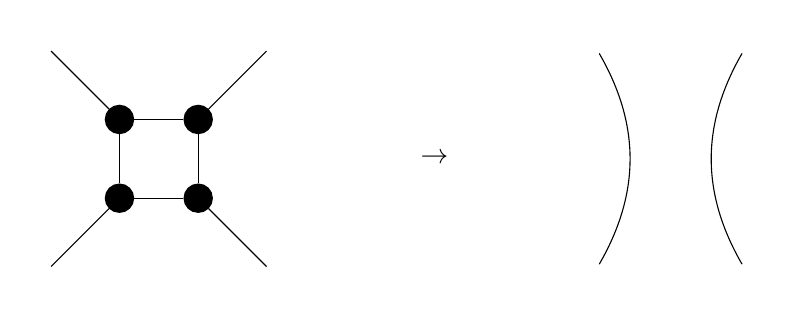
\begin{tikzpicture}[every node/.style={draw,circle,very thick, fill=black}]
	
	\node[draw=none, fill=none] (1) at (0,0) {};
	\node[draw=none, fill=none] (2) at (3,0) {};
	\node[draw=none, fill=none] (3) at (0,3) {};
	\node[draw=none, fill=none] (4) at (3,3) {};
	\node (5) at (1,1) {};
	\node (6) at (2,1) {};
	\node (7) at (1,2) {};
	\node (8) at (2,2) {};
	
	\path (1) edge (5);
	\path (2) edge (6);
	\path (3) edge (7);
	\path (4) edge (8);
	\path (5) edge (6);
	\path (5) edge (7);
	\path (8) edge (6);
	\path (8) edge (7);
	
	\node[draw=none, fill=none] (arrow) at (5, 1.5) {$\rightarrow$};
	
	\node[draw=none, fill=none] (9) at (7,0) {};
	\node[draw=none, fill=none] (10) at (9,0) {};
	\node[draw=none, fill=none] (11) at (7,3) {};
	\node[draw=none, fill=none] (12) at (9,3) {};
	
	\path (9) edge[bend right] (11);
	\path (10) edge[bend left] (12);

	
	
\end{tikzpicture}
	\caption{Replacement of a quadrilateral in a snark}
	\label{fig:trivial-quadrilateral}
\end{figure}

As mentioned before, a cubic graph with a bridge is uncolourable. If a graph has cyclic edge connectivity 1, it is clear that it has a bridge, thus, is uncolourable. Because of that, we consider the cubic graphs with cyclic edge connectivity 1 as trivial snarks. Now let us consider a snark $G$ with cyclic edge connectivity 2. That means it has a~2-edge-cut, decomposing it into two 2-poles, $M$ and $N$. We show that at least one of them is uncolourable. Suppose that both are colourable. Because of the Parity Lemma, both semiedges in $M$ and $N$ have the same colour, so after the junction of $S(M)$ and $S(N)$, we obtain $G$, which would be colourable and that is impossible. Therefore at least one of them is uncolourable, which means we can obtain a new smaller snark by the junction of the two semiedges in the uncolourable 2-pole.

Assume that a snark $G$ has cyclic edge connectivity $3$. As before, at least one of the components $M, N$ obtained by severing the edges in the 3-edge-cut of $G$ must be uncolourable, otherwise, all three semiedges of $M$ and $N$ would have three different colours because of the Parity Lemma, and thus the colouring of $G$ could be obtained. This means that we can construct a smaller snark by joining the semiedges of the~uncolourable component in a new vertex.

In our work, a snark is considered trivial if a new smaller snark can be obtained using one of the methods mentioned above in this chapter. Now we can adequately define when a snark is nontrivial.

\begin{definition}
	A snark is called \textit{nontrivial} if it has girth at least five and is cyclically 4-edge-connected. Otherwise, it is called \textit{trivial}.
\end{definition}